\subsection{Approach for Deepfake Detection}

For deepfake detection, our approach combines the power of vision transformers with advanced techniques in computer vision. Vision transformers excel in capturing both global and local features within an image, making them suitable for identifying subtle inconsistencies introduced by deepfake manipulation.
\\
\\
Our approach involves the following steps:

\noindent\textbf{Dataset Collection:} We gather a diverse dataset comprising real and deepfake images. This dataset is crucial for training and evaluating our deepfake detection model.
\\

\noindent \textbf{Vision Transformer Architecture:} We chose the Vision Transformer (ViT) architecture due to its ability to process image patches and learn relationships between them using self-attention mechanisms. ViT has shown impressive results in various computer vision tasks, and we adapt it for deepfake detection.
\\

\noindent\textbf{Preprocessing:} We preprocess the dataset to extract image patches and resize them to a consistent input size. These patches retain essential information while reducing computational complexity. Additionally, we normalize pixel values to ensure consistent input for the model.
\\

\noindent\textbf{Training:} During training, our vision transformer learns to differentiate between real and manipulated images. We use a binary cross-entropy loss function to optimize the model's weights. The self-attention mechanism in the ViT helps the model focus on relevant patches and capture intricate patterns indicative of deepfake manipulation.
\\

\noindent\textbf{Evaluation:} We evaluate the model's performance using various metrics such as accuracy, precision, recall, and F1-score. These metrics provide insights into how effectively the model distinguishes between real and deepfake images.
\\
\newpage
\noindent\textbf{Vision Transformer Architecture:}

\noindent The Vision Transformer (ViT) architecture comprises the following components:
\\

\noindent \textit{Patch Embedding:} Input images are divided into non-overlapping patches. Each patch is linearly projected to obtain embeddings, which are then augmented with positional encodings to maintain spatial information.
\\

\noindent \textit{Transformer Encoder:} The patch embeddings are fed into a stack of transformer encoder layers. Each layer consists of multi-head self-attention and feedforward neural networks. This enables the model to capture both local and global dependencies within the image.
\\

\noindent \textit{Classification Head:} The final layer of the model serves as the classification head. It takes the transformed embeddings and predicts whether an image is real or manipulated.
\\

\begin{figure}[h]
    \centering
    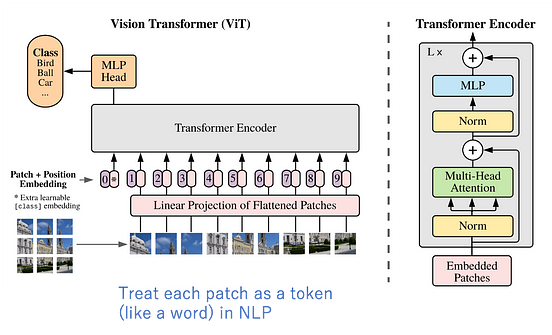
\includegraphics[width=6in]{img/visiontransformer.png}
    \caption{Vision Transformer Architecture}
\end{figure}

\newpage
\noindent \textbf{Steps:}
\vspace{0.2cm}

\noindent \textbf{Dataset Overview:}

\noindent Our dataset includes a diverse collection of real and deepfake images sourced from various public datasets and proprietary sources. It covers a wide range of scenarios, lighting conditions, and facial expressions to ensure the model's robustness.
\\

\noindent \textbf{Preprocessing Techniques:}

\noindent Before training the model, we preprocess the dataset as follows:
\\

\noindent \textit{Resize:} All images are resized to a consistent resolution, e.g., 224x224 pixels, to ensure uniform input size for the vision transformer.
\\

\noindent \textit{Augmentation:} We apply data augmentation techniques such as random rotations, flips, and brightness adjustments to increase the dataset's diversity and improve generalization.
\\

\noindent By preprocessing the dataset, we enhance the model's ability to learn relevant features and patterns necessary for accurate deepfake detection.

\noindent This approach leverages the capabilities of vision transformers while customizing them for the specific challenges posed by deepfake detection. It combines the strengths of both the architecture and the preprocessing techniques to build a robust and efficient deepfake detection model.

